\chapter{Added Components}
In this chapter each component will be discussed with more detail, such as used technology and how does component map to docker containers
\section{SimBaD-Client}
From user perspective, the SimBaD-Client is the central point of the application. In this sec
The second section will talk about the two main application views- the configuration editor and the simulation pipeline view. Finally, the way of serving application will be discussed and what will be placed in docker container responsible for SimBaD-Client.
\subsection{Technology}
\subsubsection{Overview of frameworks}
The web development ecosystem in current year is as rich as it is complicated.  For anything other than a simple static website, many tools are necessary to solve problems such as making the website work in different browsers, internationalization, or production and development builds. There are numerous frontend JavaScript frameworks, such as Angular, React or Vue to name a few. One can achieve exactly the same result using those frameworks, so the choice between mainly comes down to developer preference. For the SimBaD-Client, Angular is the framework of choice, due to its excellent support for Typescript, tooling with Angular-CLI, great UI library - Angular Material and OpenApi Codegen support, used to generate client libraries communicating with SimBaD-Pipeline-Server API. 
\subsubsection{Monorepo pattern}
The project was bootstrapped with Angular-CLI and NX using monorepo pattern. Monorepo, is a pattern that helps organize and share code between multiple JavaScript applications. Code in monorepo, as the name indicates is put in single repository. Monorepo ensures that everything at a single commit works together - for code in separate repositories, the state of application is a combination of several commits from each repository. Another benefit, especially important for frontend applications, is that it allows to centralize the build system and and tool chain - all of the code in monorepo is build using Angular-CLI and depends on same libraries. It makes easy to split the code into libraries, and to compose applications using those libraries. For SimBaD-Client it allows to split the client code into apps, such as SimBaD-Client app, developer server for building frontend independently from backend, and shared API and UI libraries. The CI process is also simplified, as each change and applications and libraries that are affected by this change can be tested, and pass for such tests proves that each application in monorepo works as indented.
\subsubsection{Reactive programming and store architecture}
Reactive programming is a programming paradigm that deals with asynchronous data streams - sequences of some kind of events ordered in time. Data streams can be created from anything, from click events, http calls to user inputs or variable declarations. Streams can be then manipulated, for example they can be filtered, merged, mapped to other streams. Those streams can also be "subscribed to" or "consumed" to produce some kind of side effect, like showing notification in UI, when some API returns specific status. Reactive programming changes the way that application components communicate with each other. Instead of pushing data directly into components, or components asking explicitly for data, in reactive programming they automatically "react" to data changes. The most popular library for Reactive programming is Rx (Reactive extensions), and RxJS is the JavaScript version of this library. For web applications, when almost all code, including simple console.log() statements is executed asynchronously, and there is multitude of UI or data related Events to react to, RxJS allows to write code that handles those events in a clean, maintainable and concise way.
\begin{figure}[h!]
	\centering
		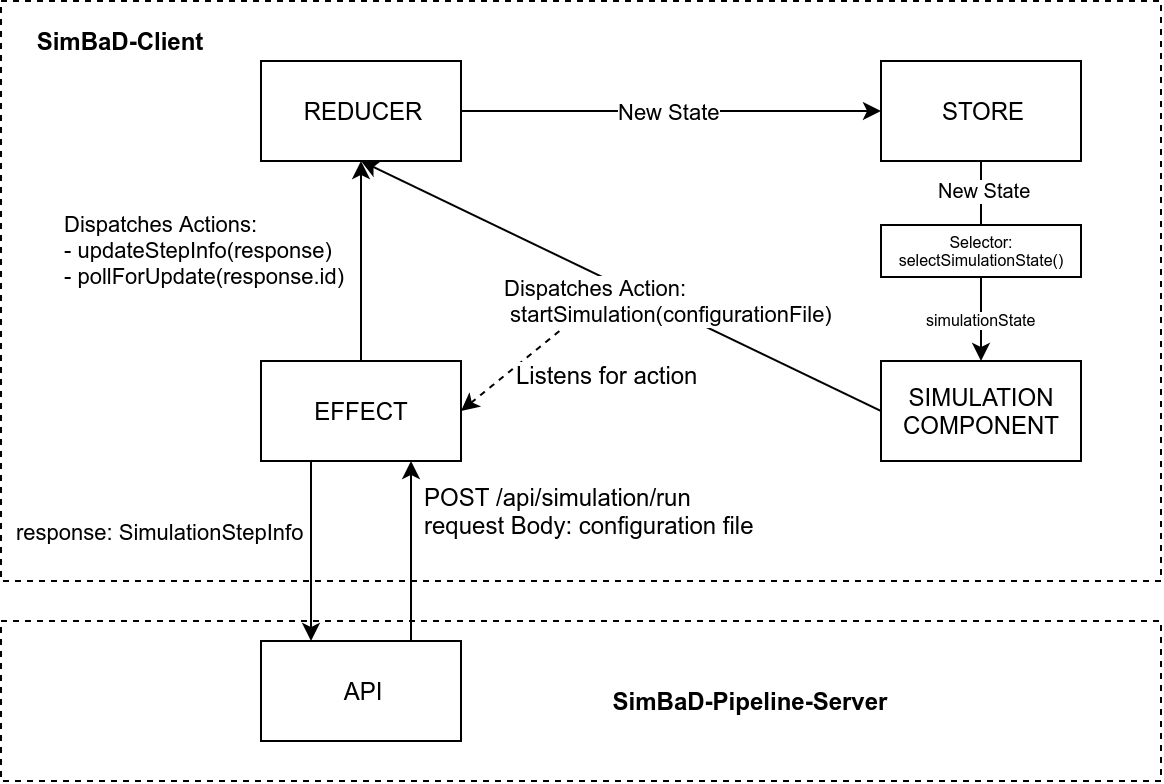
\includegraphics[width=0.9\linewidth]{diagrams/ngrx.png}
	\caption{Example of NgRX flow in SimBad-Client}
	\label{fig:ngrx}
\end{figure}
Reactive programming works very well with store architecture. The store can be thought of as a client-side database, where all data needed by application resides. The store reflects the complete state of application.
NgRX uses the RxJS library heavily - the store itself is an obervable, an components need to subscribe to the store observables to get the data. Store architecture solves problem of passing data between components.
In angular, data can be passed between components in server ways - from parent to child using Input() member variables, from child to parent using EventEmmiters() and between unrelated components using services. Problems arise when data needs to be passed several levels down in component tree - the root component has the data, and the leaf components needs this data, however for the component nodes along the way, that do not need the data, extraneous Input properties must be added. Store architecture bypasses that problem, by providing single source of truth or the store for all of the components to get data from and push data to. When actor such as user or server changes some data, this change is pushed to store, and automatically reflected in all of the components. NgRX is a library that provides tools to add store architecture to application. 
NgRx consists of several building blocks - actions, reducers, effects and selectors. The components can alter state of application or by dispatching actions to store. Actions consists of type - unique action identifier and payload - the data that is needed to change the state. Reducer is a pure function that accepts two arguments - current state of application and action. Reducer analyzes the action and returns new state that is a combination of previous state and action payload. Side effect can be something like making a http call, or showing a notification. The effects trigger when specific action is dispatched to store, and can be used to trigger side-effect based on those actions. Effects can also dispatch another action to the store, for example they can push response received from http call. Single effect can be triggered by multiple action, can dispatch multiple actions and single action can trigger multiple effects. The store can be pretty big object, and components need only a part of it. Selectors facilitate this by allowing the components to get or in other words "select" only parts of the store. In the figure \ref{fig:ngrx}, example NgRX flow trigerred by user starting the simulation is shown.

The user action, for example clicking a button, causes the component responsible for simulation view to dispatch startSimulation() action with simulation configuration file as its payload. This triggers two separate NgRX flows. In the first one, the action is passed to the reducer, and new state with added information that simulation has started is generated. Then the store observable emits new data and component receives a slice of this data, based on selector. The second flow starts with effect, that reacts to startSimulation Action being triggered. This effect makes then POST request to Simulation-Pipeline-Server to start simulation, and receives the information about the first simulation step - the SimBaD-CLI step. Effect then dispatches two actions with, response as a payload, one to update step info in store, and one to start polling for step info changes. Those actions then are handled by reducer, new store state is emitted and passed to component. If dispatched actions trigger any effects, another flow starts.
\subsection{Configuration Editor}
To start simulation process user needs to pass simulation configuration file or SCF. This file has tree-like structure and contains various objects and parameters that control the simulation process. Although those objects need have predefined value types, ranges, or enums, the exact definitions did not exists, and had to be created. Detailed description of this file and how to add new parameters to simulation can be found in appendix \ref{appendix:A}.
\begin{figure}[h!]
	\centering
		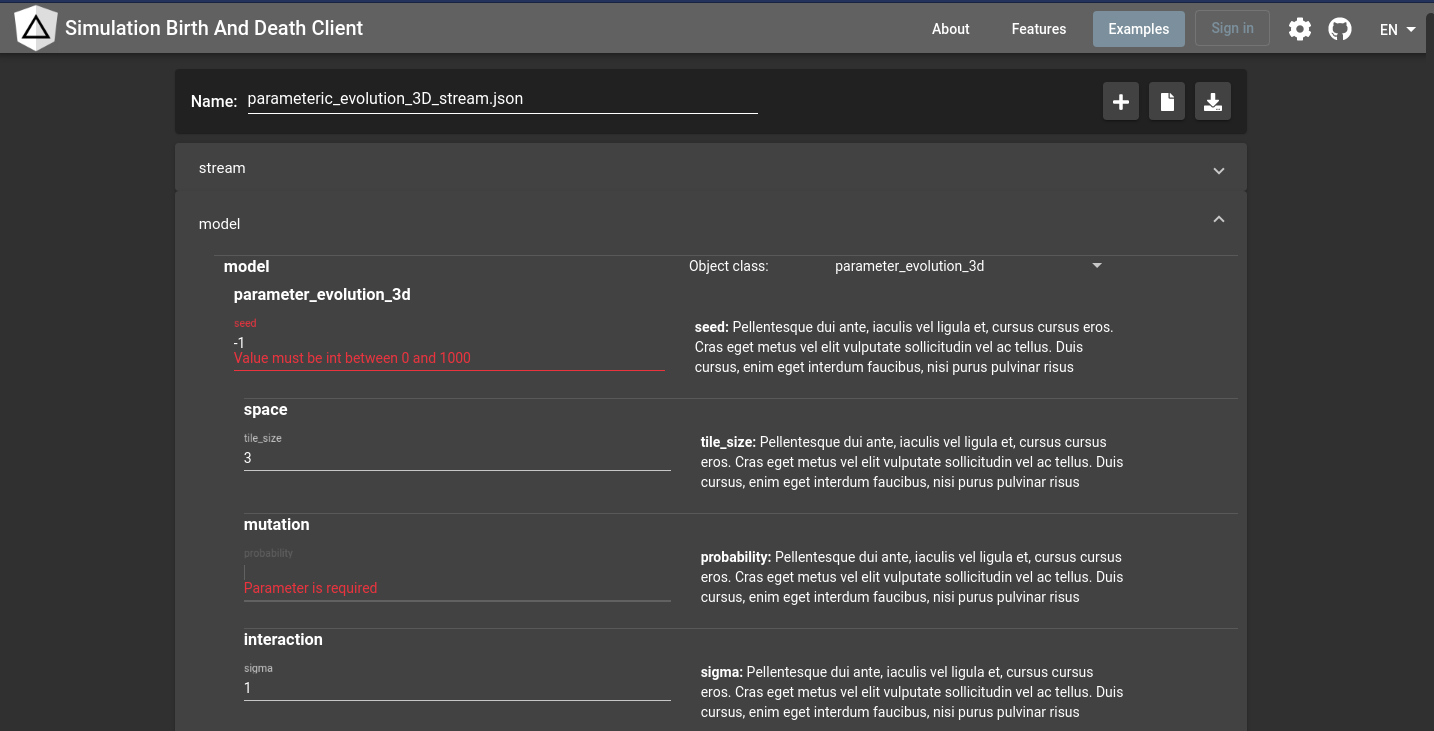
\includegraphics[width=0.9\linewidth]{screens/conf-view.png}
	\caption{The configuration editor view}
	\label{fig:conf-view}
\end{figure}
To enable user to generate valid configuration, configuration editor was created. Configuration editor generates forms that validate the parameter values entered by user against their definitions. The form has tree structure that maps to configuration. Additionally, each form input associated with parameter displays validation messages, and parameter description. The form is generated dynamically, and adding or changing definition in object definition does not break the form, though it requires to rebuild application. The user can create new configuration, and download and upload the configuration from .json file.  The SimBaD-CLI supports two file formats: .json and .simbad which is an alias to default boost:tree format. As the changes in configuration are dispatched to store, the configuration can be shared between different components. 
\begin{figure}[h!]
	\centering
		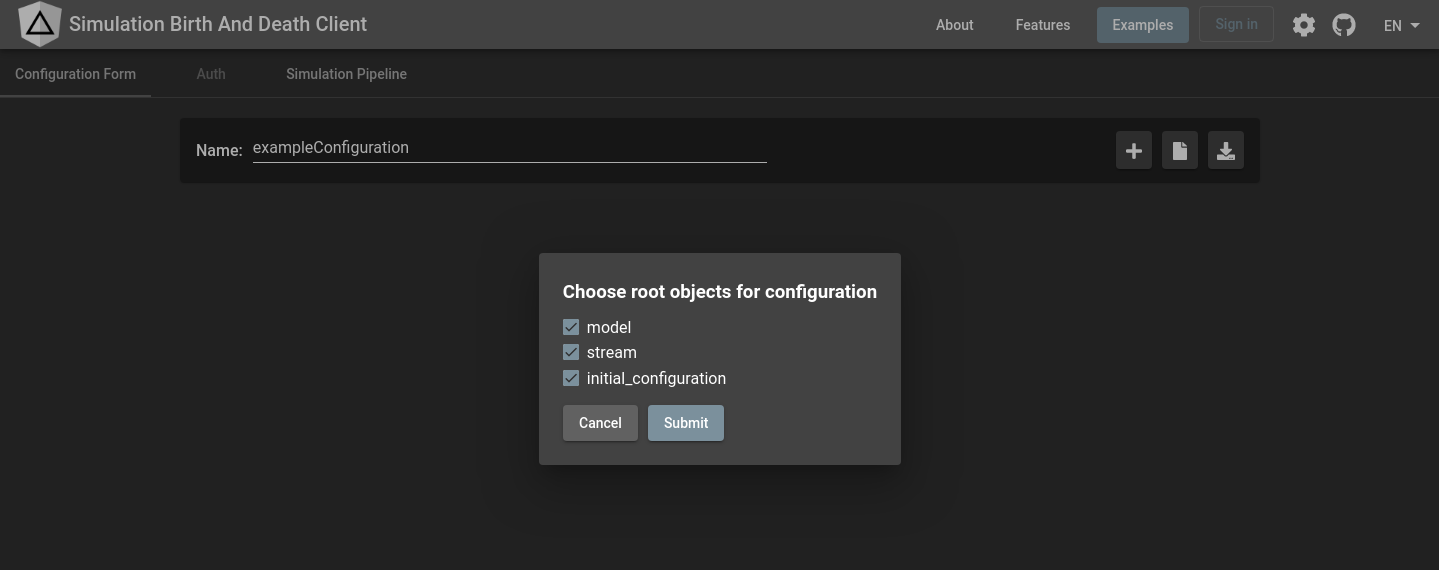
\includegraphics[width=0.9\linewidth]{screens/configuration-view-modal.png}
	\caption{Creating new configuration}
	\label{fig:conf-view-new}
\end{figure}
\subsection{Simulation Pipeline}

\section{SimBaD-Pipeline-Server}
\subsubsection{Overview of frameworks}
\subsection{Task queue}
\subsection{Task executors}
\subsection{Storing simulation Data}
\section{SimBaD-Analyzer-Server}
\subsection{Integration with spark}
\section{SimBaD-Host-Link}
\section{Docker containers for components}
\section{System Configuration}